\documentclass{article}
\usepackage{graphicx}
\usepackage{amsmath}
\usepackage{booktabs}
\usepackage{array}
\usepackage{hyperref}
\usepackage{float}
\usepackage{tikz}
\usepackage{circuitikz}
\usepackage{karnaugh-map}
\usepackage{subcaption}


\title{\textbf{Lab Report: Experiment 7}}
\author{EE24BTECH11003 : Akshara Sarma Chennubhatla\\EE24BTECH11005 : Arjun Pavanje}

\begin{document}
\maketitle
\begin{center}
	\textbf{Experiment:}\\Designing an asynchronous\\mod 7 counter using\\T Flip-Flops 
\end{center}
\vspace{30pt}
\begin{figure}[h!]
	\centering
	
\includegraphics[width = 100pt]{.logo/logo.png}\\
\end{figure}
\begin{center}
	Bachelor of Technology\\
	\vspace{10pt}
	Department of Electrical Engineering\\
\end{center}
\newpage


\section{Introduction}

This experiment focuses on designing and implementing a Mod-7 asynchronous counter using T flip-flops, using clock from an Arduino.

\section{Theory}
\subsection{T Flip-Flop}

\begin{figure}[!ht]
\centering
\resizebox{0.6\textwidth}{!}{%
\begin{circuitikz}
\tikzstyle{every node}=[font=\large]
\draw  (6.25,13) rectangle (8.75,10.5);
\draw [short] (6.25,12.5) -- (5,12.5);
\draw [short] (6.25,11) -- (5,11);
\draw [short] (8.75,12.5) -- (10,12.5);
\draw [short] (8.75,11) -- (10,11);
\node [font=\normalsize] at (4.2,12.5) {Input};
\node [font=\normalsize] at (4.25,11) {Clock};
\node [font=\large] at (6.75,12.5) {\textbf{T}};
\node [font=\large] at (7,11) {\textbf{CLK}};
\node [font=\large] at (8.4,12.5) {\textbf{Q}};
\node [font=\large] at (8.4,11) {$\mathbf{\overline{Q}}$};
\end{circuitikz}
}%

\label{fig:my_label}
\end{figure}

The Toggle Flip-Flop also known as T Flip-Flop is a type of Flip-Flop in which the output takes in the input value if the state of T is high (T = 0) and takes the value of the complement of the input if T is low (T = 1). This happens when the clock is high. When the clock is low, the output retains its previous state.
\begin{align*}
    Q_{n + 1} = 
    \begin{cases}
        Q_n &, T = 0\\\\
        \overline{Q_n} &, T = 1
    \end{cases}
\end{align*}
The Truth table for the Flip-Flop is,\\
\begin{table}[h]
\centering
\begin{tabular}{|c|c|c|}
\hline
$T$ & $Q_n$ & $Q_{n+1}$ \\
\hline
0 & 0 & 0 \\
0 & 1 & 1 \\
1 & 0 & 1 \\
1 & 1 & 0 \\
\hline
\end{tabular}
\end{table}

The internal Circuit diagram of the T Flip-Flop is given below,
\pagebreak
\begin{figure}[h!]
\centering
\resizebox{1\textwidth}{!}{%
\begin{circuitikz}
\tikzstyle{every node}=[font=\large]
\draw (7.5,14.5) to[short] (7.75,14.5);
\draw (7.5,14) to[short] (7.75,14);
\draw (7.75,14.5) node[ieeestd and port, anchor=in 1, scale=0.89](port){} (port.out) to[short] (9.5,14.25);
\draw (port.left) to[short] (7.5,14.25);
\draw (7.5,10.75) to[short] (7.75,10.75);
\draw (7.5,10.25) to[short] (7.75,10.25);
\draw (7.75,10.75) node[ieeestd and port, anchor=in 1, scale=0.89](port){} (port.out) to[short] (9.5,10.5);
\draw (port.left) to[short] (7.5,10.5);
\draw (12.5,14.25) to[short] (12.75,14.25);
\draw (12.5,13.75) to[short] (12.75,13.75);
\draw (12.75,14.25) node[ieeestd nor port, anchor=in 1, scale=0.89](port){} (port.out) to[short] (14.5,14);
\draw (12.5,11) to[short] (12.75,11);
\draw (12.5,10.5) to[short] (12.75,10.5);
\draw (12.75,11) node[ieeestd nor port, anchor=in 1, scale=0.89](port){} (port.out) to[short] (14.5,10.75);
\draw (9.5,10.5) to[short] (12.5,10.5);
\draw (9.5,14.25) to[short] (12.5,14.25);
\draw (7.5,14) to[short] (6.25,14);
\draw (6.25,14) to[short] (6.25,10.75);
\draw (7.5,10.75) to[short] (6.25,10.75);
\draw (7.5,14.25) to[short] (3.75,14.25);
\draw (3.75,14.25) to[short] (3.75,10.5);
\draw (7.5,10.5) to[short] (3.75,10.5);
\draw (14.5,10.75) to[short] (17,10.75);
\draw (14.5,14) to[short] (17,14);
\draw (15,14) to[short] (12.5,11.5);
\draw (12.5,11.5) to[short] (12.5,11);
\draw (15,10.75) to[short] (12.5,13.25);
\draw (12.5,13.25) to[short] (12.5,13.75);
\draw (7.5,14.5) to[short] (7.5,15.25);
\draw (7.5,15.25) to[short] (16.25,15.25);
\draw (16.25,15.25) to[crossing] (16.25,12.75);
\draw (16.25,12.75) to[short] (16.25,10.75);
\draw (7.5,10.25) to[short] (7.5,9.75);
\draw (7.5,9.75) to[short] (15.75,9.75);
\draw (15.75,9.75) to[crossing] (15.75,11.75);
\draw (15.75,11.75) to[short] (15.75,14);
\draw (6.25,12.5) to[short, -o] (5.25,12.5) ;
\draw (3.75,10.5) to[short, -o] (2.75,10.5) ;
\node [font=\large] at (2.25,10.5) {\textbf{T}};
\node [font=\large] at (4.5,12.5) {\textbf{CLK}};
\draw (16.5,14) to[short, -o] (17.5,14) ;
\draw (17,10.75) to[short, -o] (17.5,10.75) ;
\node [font=\large] at (18,14) {\textbf{Q}};
\node [font=\large] at (18.25,10.75) {$\mathbf{\overline{Q}}$};
\end{circuitikz}
}%

\label{fig:my_label}
\end{figure}

\subsection{JK Flip-Flop}

\begin{figure}[!ht]
\centering
\resizebox{0.5\textwidth}{!}{%
\begin{circuitikz}
\tikzstyle{every node}=[font=\large]
\draw  (6.25,14.25) rectangle (11.25,9.25);
\draw [short] (6.25,13) -- (5,13);
\draw [short] (6.25,11.75) -- (5,11.75);
\draw [short] (6.25,10.5) -- (5,10.5);
\draw [short] (11.25,13) -- (12.5,13);
\draw [short] (11.25,10.5) -- (12.5,10.5);
\node [font=\large] at (6.75,13) {\textbf{J}};
\node [font=\large] at (6.75,10.5) {\textbf{K}};
\node [font=\large] at (7,11.75) {\textbf{CLK}};
\node [font=\large] at (10.75,13) {\textbf{Q}};
\node [font=\large] at (10.75,10.5) {$\mathbf{\overline{Q}}$};
\end{circuitikz}
}%

\label{fig:my_label}
\end{figure}

The JK Flip-Flop works on the principle that the output is equal to the input when both J and K are low (J = K = 0). The output takes the value of the complement of the input if both J and K are high (J = K = 1). In any other case, the output takes the value of J regardless of K. This happens when the clock is high. When the clock is low, the output retains its previous state.

\begin{align*}
    Q_{n + 1} = 
    \begin{cases}
        Q_n &, J = 0, K = 0\\\\
        \overline{Q_n} &, J = 1, K = 1\\\\
        0 &, J = 0, K = 1\\\\
        1 &, J = 1, K = 0
    \end{cases}
\end{align*}

The truth table of the JK Flip-Flop is given below,\\
\pagebreak
\begin{table}[h!]
\centering
\begin{tabular}{|c|c|c|c|}
\hline
$J$ & $K$ & $Q_n$ & $Q_{n+1}$ \\
\hline
0 & 0 & 0 & 0 \\
0 & 0 & 1 & 1 \\
0 & 1 & 0 & 0 \\
0 & 1 & 1 & 0 \\
1 & 0 & 0 & 1 \\
1 & 0 & 1 & 1 \\
1 & 1 & 0 & 1 \\
1 & 1 & 1 & 0 \\
\hline
\end{tabular}
\end{table}

The internal circuit diagram of the JK Flip-Flop is as below,\\

\begin{figure}[h!]
\centering
\resizebox{1\textwidth}{!}{%
\begin{circuitikz}
\tikzstyle{every node}=[font=\large]
\draw (9.5,10.5) to[short] (12.5,10.5);
\draw (9.5,14.25) to[short] (12.5,14.25);
\draw (7.5,14) to[short] (6.25,14);
\draw (6.25,14) to[short] (6.25,10.75);
\draw (7.5,10.75) to[short] (6.25,10.75);
\draw (14.5,10.75) to[short] (17,10.75);
\draw (14.5,14) to[short] (17,14);
\draw (15,14) to[short] (12.5,11.5);
\draw (12.5,11.5) to[short] (12.5,11);
\draw (15,10.75) to[short] (12.5,13.25);
\draw (12.5,13.25) to[short] (12.5,13.75);
\draw (7.5,14.5) to[short] (7.5,15.25);
\draw (7.5,15.25) to[short] (16.25,15.25);
\draw (16.25,15.25) to[crossing] (16.25,12.75);
\draw (16.25,12.75) to[short] (16.25,10.75);
\draw (7.5,10.25) to[short] (7.5,9.75);
\draw (7.5,9.75) to[short] (15.75,9.75);
\draw (15.75,9.75) to[crossing] (15.75,11.75);
\draw (15.75,11.75) to[short] (15.75,14);
\draw (6.25,12.5) to[short, -o] (5.25,12.5) ;
\node [font=\large] at (4.5,12.5) {\textbf{CLK}};
\draw (16.5,14) to[short, -o] (17.5,14) ;
\draw (17,10.75) to[short, -o] (17.5,10.75) ;
\node [font=\large] at (18,14) {\textbf{Q}};
\node [font=\large] at (18.25,10.75) {$\mathbf{\overline{Q}}$};
\draw (7.5,14.5) to[short] (7.75,14.5);
\draw (7.5,14) to[short] (7.75,14);
\draw (7.75,14.5) node[ieeestd nand port, anchor=in 1, scale=0.89](port){} (port.out) to[short] (9.5,14.25);
\draw (port.left) to[short] (7.5,14.25);
\draw (7.5,10.75) to[short] (7.75,10.75);
\draw (7.5,10.25) to[short] (7.75,10.25);
\draw (7.75,10.75) node[ieeestd nand port, anchor=in 1, scale=0.89](port){} (port.out) to[short] (9.5,10.5);
\draw (port.left) to[short] (7.5,10.5);
\draw (12.5,14.25) to[short] (12.75,14.25);
\draw (12.5,13.75) to[short] (12.75,13.75);
\draw (12.75,14.25) node[ieeestd nand port, anchor=in 1, scale=0.89](port){} (port.out) to[short] (14.5,14);
\draw (12.5,11) to[short] (12.75,11);
\draw (12.5,10.5) to[short] (12.75,10.5);
\draw (12.75,11) node[ieeestd nand port, anchor=in 1, scale=0.89](port){} (port.out) to[short] (14.5,10.75);
\draw (7.5,14.25) to[short] (6.25,14.25);
\draw (7.75,10.5) to[short] (6.25,10.5);
\draw (6.25,14.25) to[short, -o] (5.25,14.25) ;
\draw (6.25,10.5) to[short, -o] (5.5,10.5) ;
\node [font=\large] at (4.75,14.25) {\textbf{J}};
\node [font=\large] at (5,10.5) {\textbf{K}};
\end{circuitikz}
}%

\label{fig:my_label}
\end{figure}

\subsection{JK to T Flip-Flop Conversion}
Since JK flip-flops were provided instead of T flip-flops, conversion was necessary. Converting a JK flip-flop to a T flip-flop can be done by simply shorting J and K ports of JK flip-flops.
\begin{displaymath}
\begin{array}{|c| c|c|c |c|}
\hline
T & Q_n & Q_{n+1} & J & K \\
\hline
0 & 0 & 0 & 0 & X \\
0 & 1 & 1 & X & 0 \\
1 & 0 & 1 & 1 & X \\
1 & 1 & 0 & X & 1 \\
\hline
\end{array}
\end{displaymath}
Writing Karnaugh-map for $J$
\begin{center}
\begin{karnaugh-map}[2][2][1][$Q_n$][$T$]
    \manualterms{0,X,1,X}
    \implicant{2}{3}
    %\implicant{5}{15}
    %\implicantedge{1}{3}{9}{11}
    %\implicantcorner
    %\implicantedge{4}{12}{6}{14}
\end{karnaugh-map}
\end{center}
We get,
\begin{align*}
    J = T
\end{align*}
Now writing karnaugh-map for $K$,
\begin{center}
\begin{karnaugh-map}[2][2][1][$Q_n$][$T$]
    \manualterms{X,0,X,1}
    \implicant{2}{3}
    %\implicant{5}{15}
    %\implicantedge{1}{3}{9}{11}
    %\implicantcorner
    %\implicantedge{4}{12}{6}{14}
\end{karnaugh-map}
\end{center}
We get,
\begin{align*}
    K = T
\end{align*}
\subsection{Asynchronous Counter}
In an asynchronous counter, the clock input of each flip-flop (except the first) is driven by the output of the previous flip-flop. This creates a ripple effect as the signal propagates through the counter, hence the alternative name ``ripple counter''.

\section{Materials Required}
\begin{enumerate}
\item T flip-flops (or JK flip-flops LM7476 (or similar))
\item  NAND gate LM7410 (or similar)
\item LED
\item Arduino (for clock)
\item Oscilloscope 
\item Wires
\item Breadboard
\end{enumerate}

\section{Procedure}

\subsection{Converting JK Flip-Flops to T Flip-Flops}
Short the J and K pins of JK flip-flops as mentioned above to convert it into a T flip-flop

\subsection{Counter Design}
\begin{enumerate}
\item The PRESET pin (J) of all flip-flops was connected to \textit{HIGH}.
\item The output of the first flip-flop was connected to the clock input of the second flip-flop.
\item The output of the second flip-flop was connected to the clock input of the third flip-flop.
\item The outputs of all three flip-flops were connected to LEDs through resistors indication.
This gives a counter that goes from 0 to 7 (for the 0 to 7 counter to work, set $\mathbf{\overline{CLR}}$ to \textit{HIGH})
\end{enumerate}

\subsection{Reset Mechanism}
\begin{enumerate}
\item The outputs of all three flip-flops were connected to the inputs (1A, 1B, 1C) of the LM7410 NAND gate.
\item The output of the NAND gate (1Y) was connected to the $\mathbf{\overline{CLR}}$ pins of all flip-flops.
\end{enumerate}

This configuration ensures that when the counter reaches the state $111$ (decimal 7), the NAND gate outputs a LOW signal, which clears all flip-flops, resetting the counter to 000'' (decimal 0).

\subsection{Logic}
The output of one of the first Flip-Flop is connected to the clock of the second flip-flop. Since both J and K are 1, i.e., T = 1, output of first flip-flop will take the value of complement of its previous output at every falling edge. Similarly, for the second and the third flip-flop. But after 6 cycles of the clock, on the seventh cycle when all the 3 outputs are 1, the NAND gate to which these 3 are given as inputs takes the value 0 which is then given to the $\mathbf{\overline{CLR}}$ of the flip-flops which then sets all the outputs to 0 regardless of the inputs effectively looping it back to 0. So here, all the output signals suddenly drop to 0 from their previous state. So the graph of the outputs looks like the following plot. The period of every output signal is 7 times the time period of the clock.

\begin{figure}[h!]
    \centering
    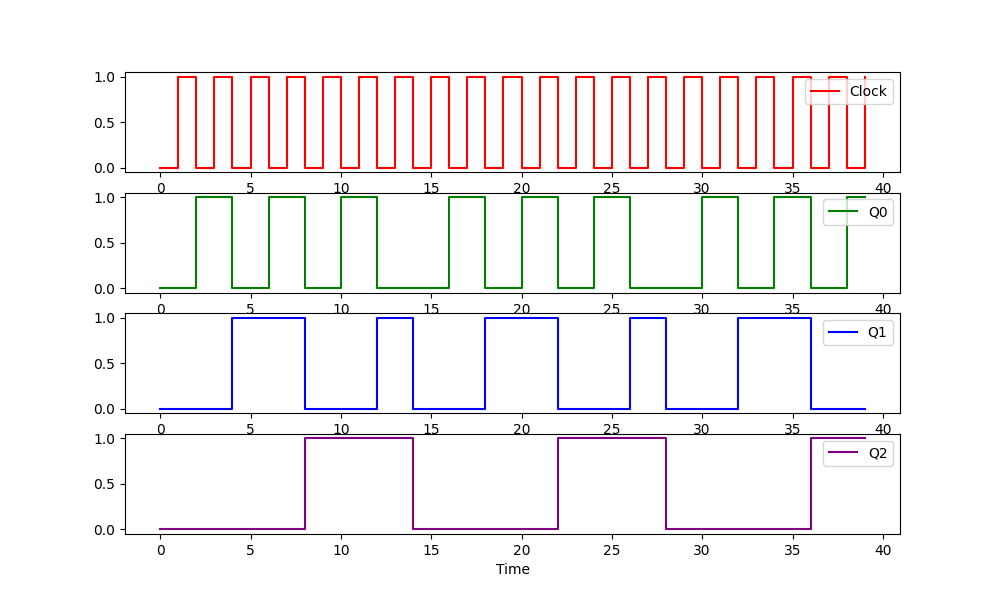
\includegraphics[width=1\linewidth]{figs/Output_signals.png}
    \caption{Clock and Output Signals}
    \label{fig:enter-label}
\end{figure}

\subsection{Clock Signal Generation}
The Arduino code used for generating a clock signal of period $1s$ is as follows:
\begin{verbatim}
    void setup () {
        pinMode(13, OUTPUT);
    }

    void loop () {
        digitalWrite(13, HIGH);
        delay(1000);
        digitalWrite(13, LOW);
        delay(1000);
    }
\end{verbatim}
\pagebreak
\subsection{Circuit Image}
\begin{figure}[h!]
    \centering
    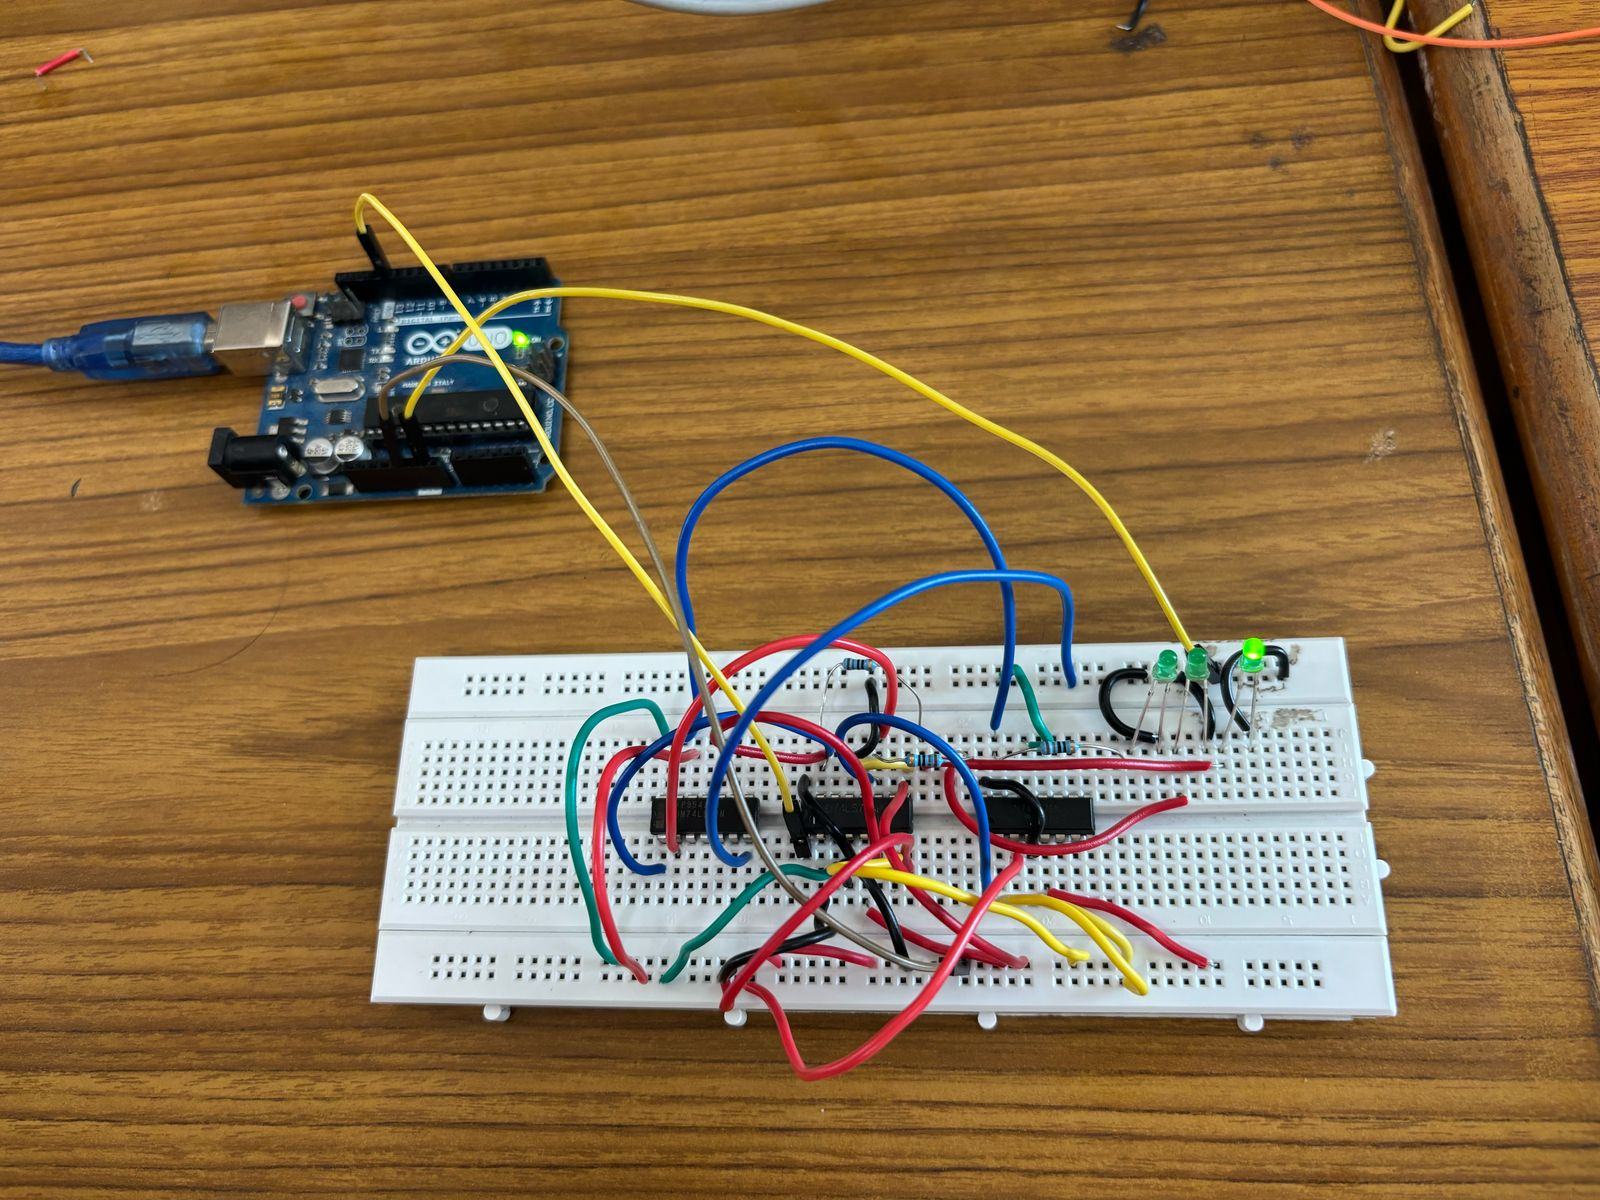
\includegraphics[width=0.7\linewidth]{figs/circuit.png}
    \caption{Circuit}
    \label{fig:enter-label}
\end{figure}

\section{Results and Observations}
\subsection{Counter}
\begin{figure}[h!]
	\begin{subfigure}[b]{100pt}
		\caption{0}
		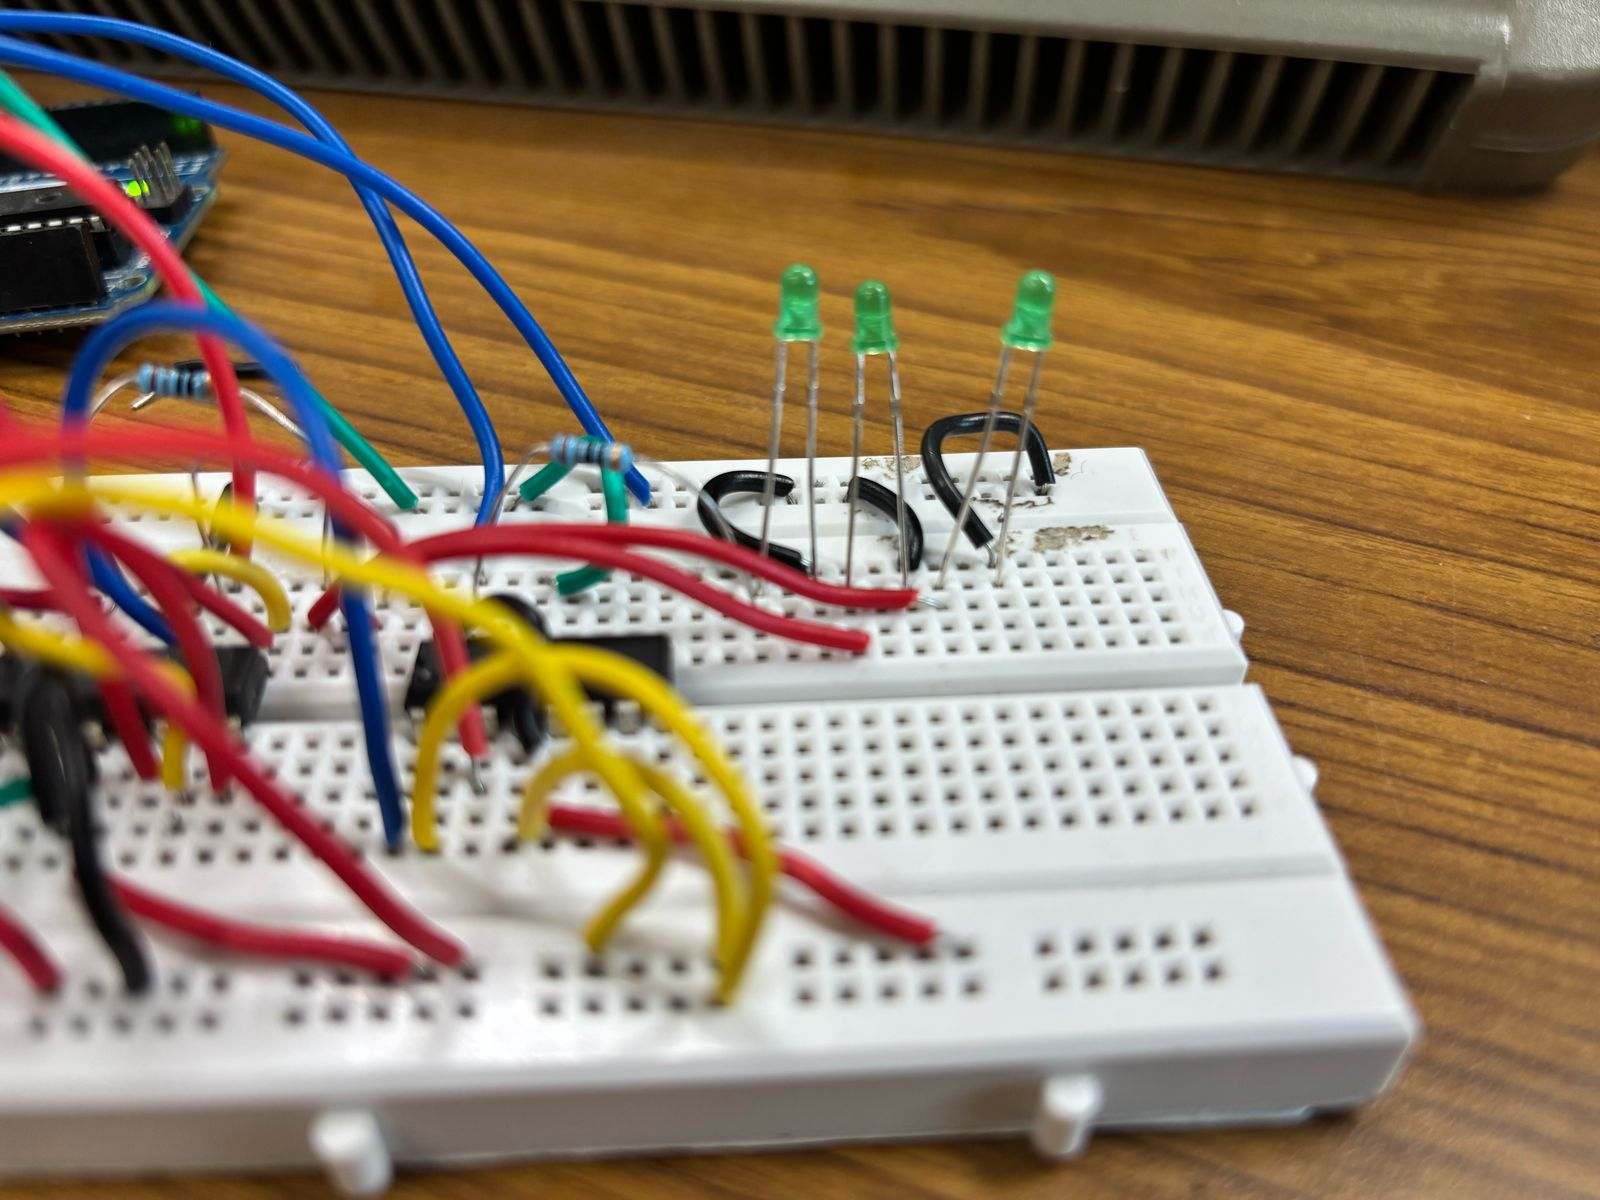
\includegraphics[width = 200pt]{figs/0.png}
	\end{subfigure}
	\hspace{110pt}
	\begin{subfigure}[b]{100pt}
		\caption{1}
		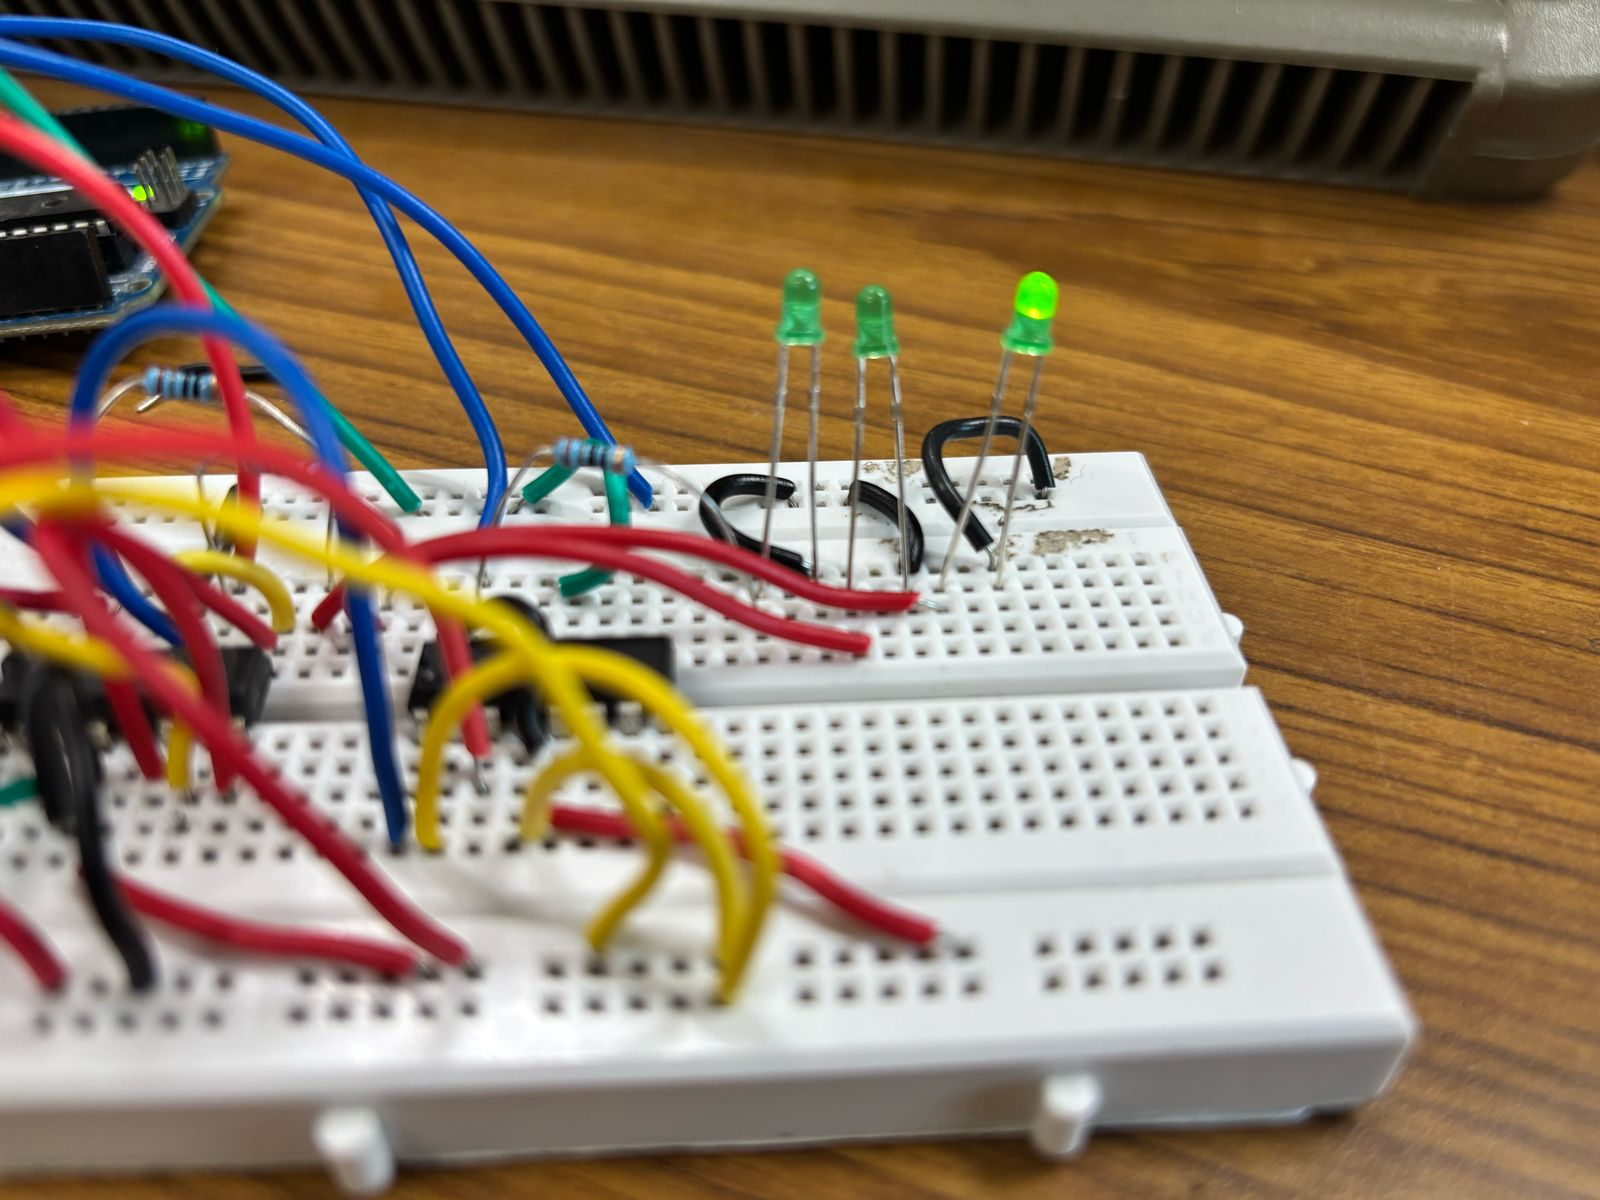
\includegraphics[width = 200pt]{figs/1.png}
	\end{subfigure}
\end{figure}
\pagebreak
\begin{figure}[h!]
    \begin{subfigure}[b]{100pt}
		\caption{2}
		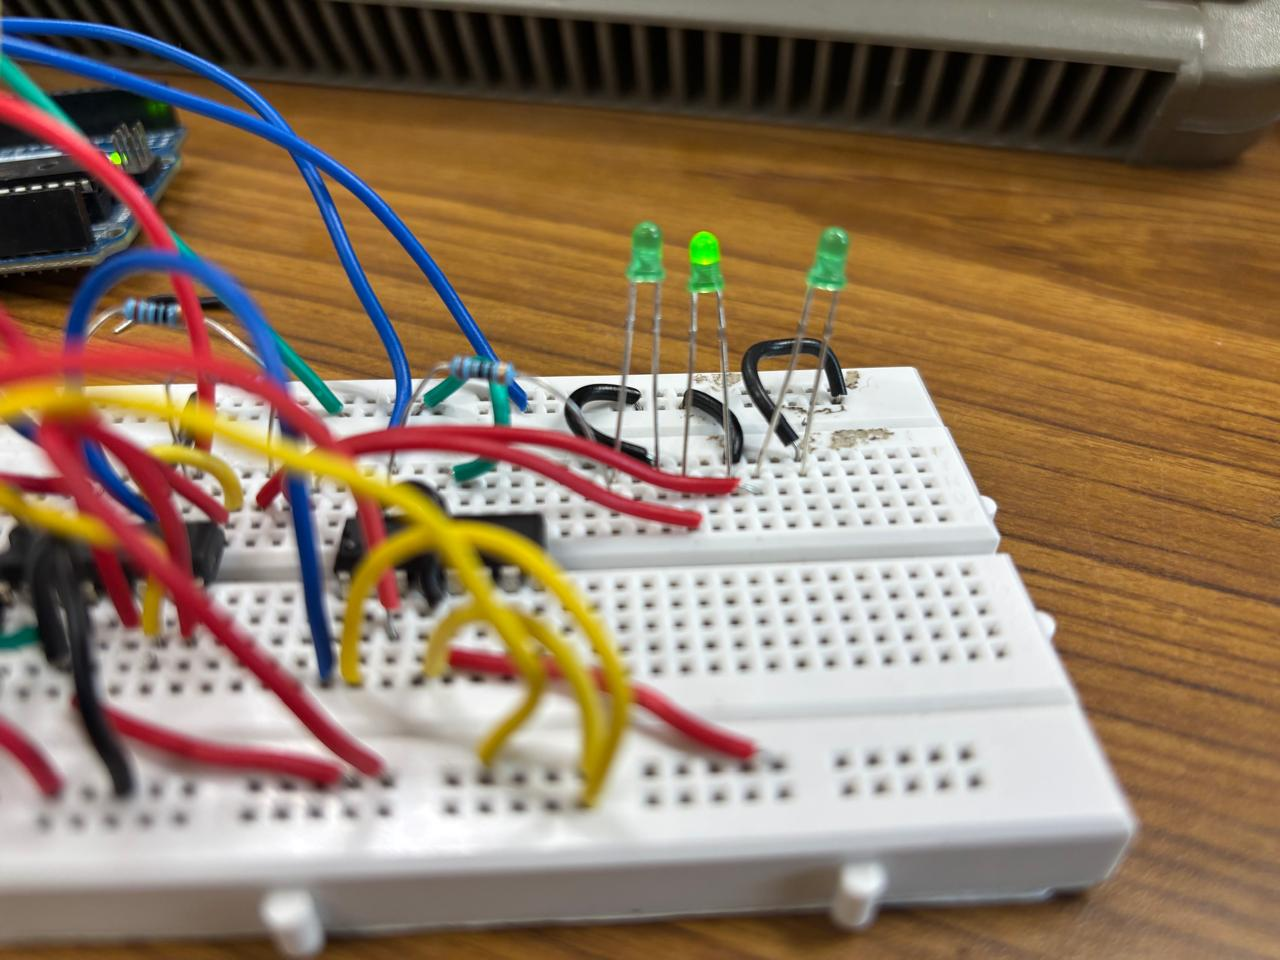
\includegraphics[width = 200pt]{figs/2.png}
	\end{subfigure}
	\hspace{110pt}
	\begin{subfigure}[b]{100pt}
		\caption{3}
		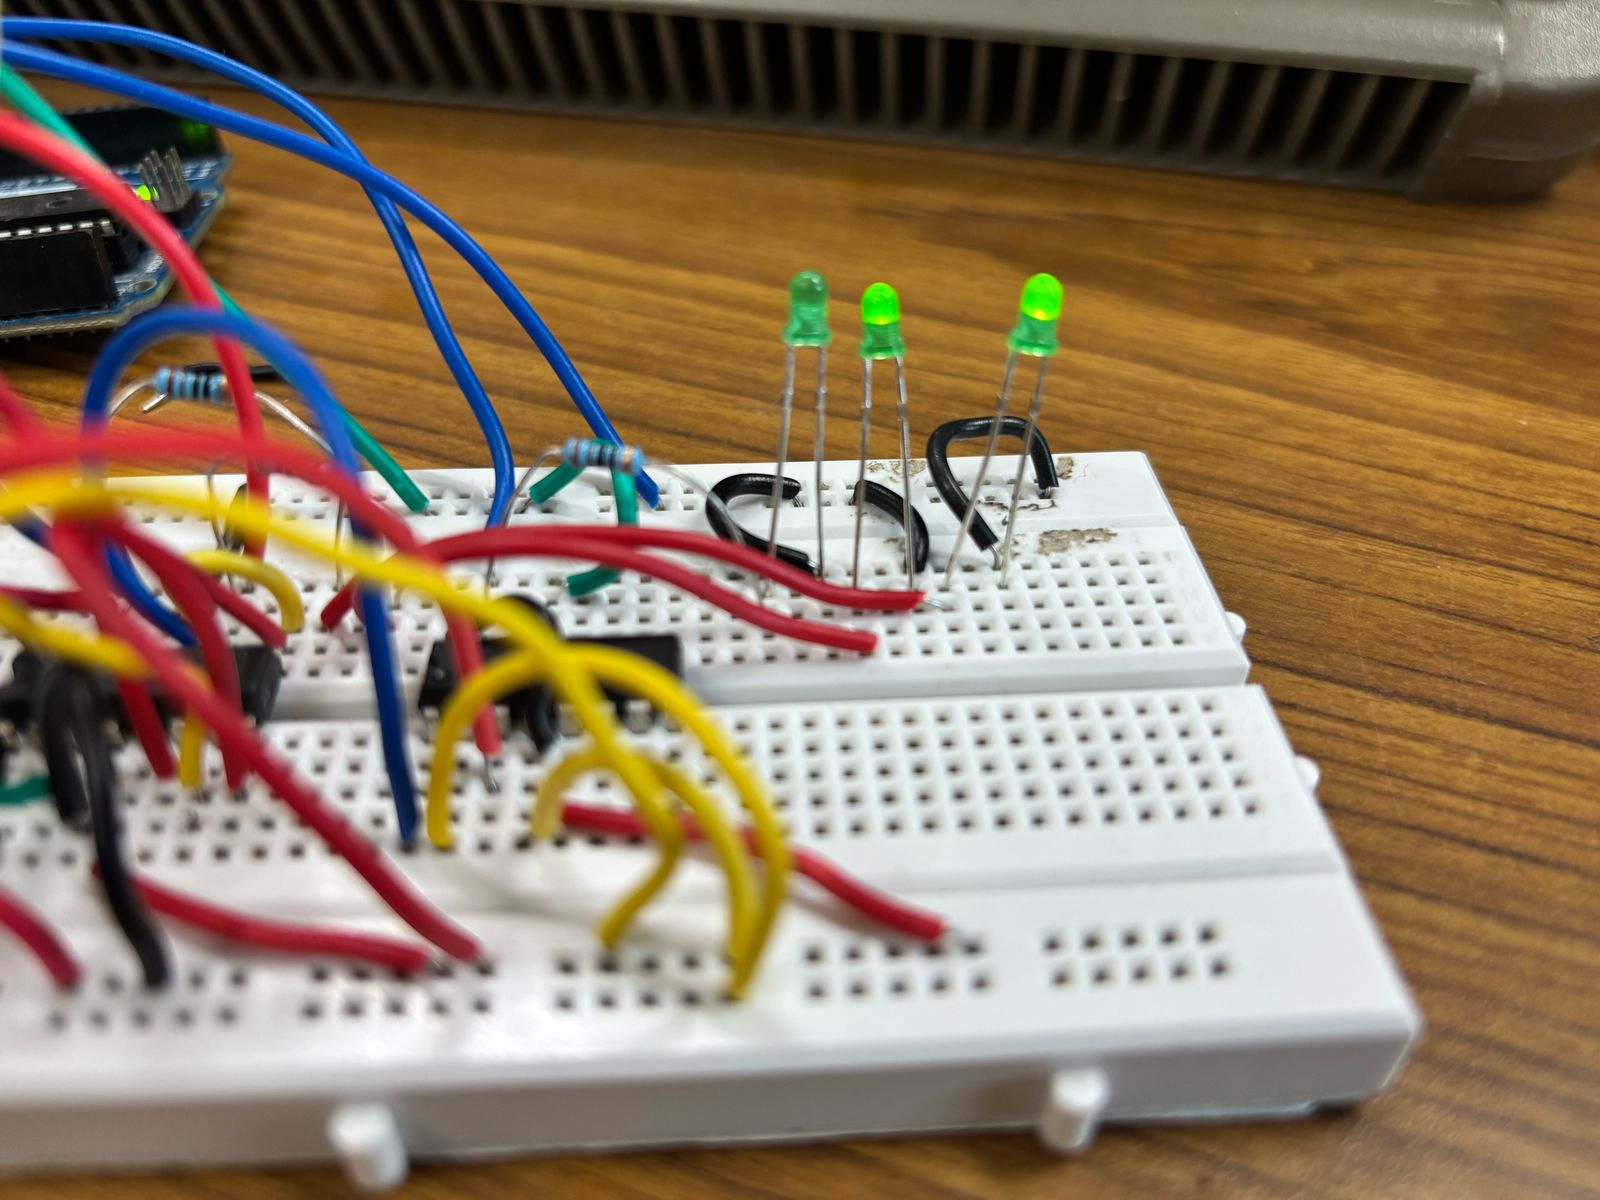
\includegraphics[width = 200pt]{figs/3.png}
	\end{subfigure}
    \begin{subfigure}[b]{100pt}
		\caption{4}
		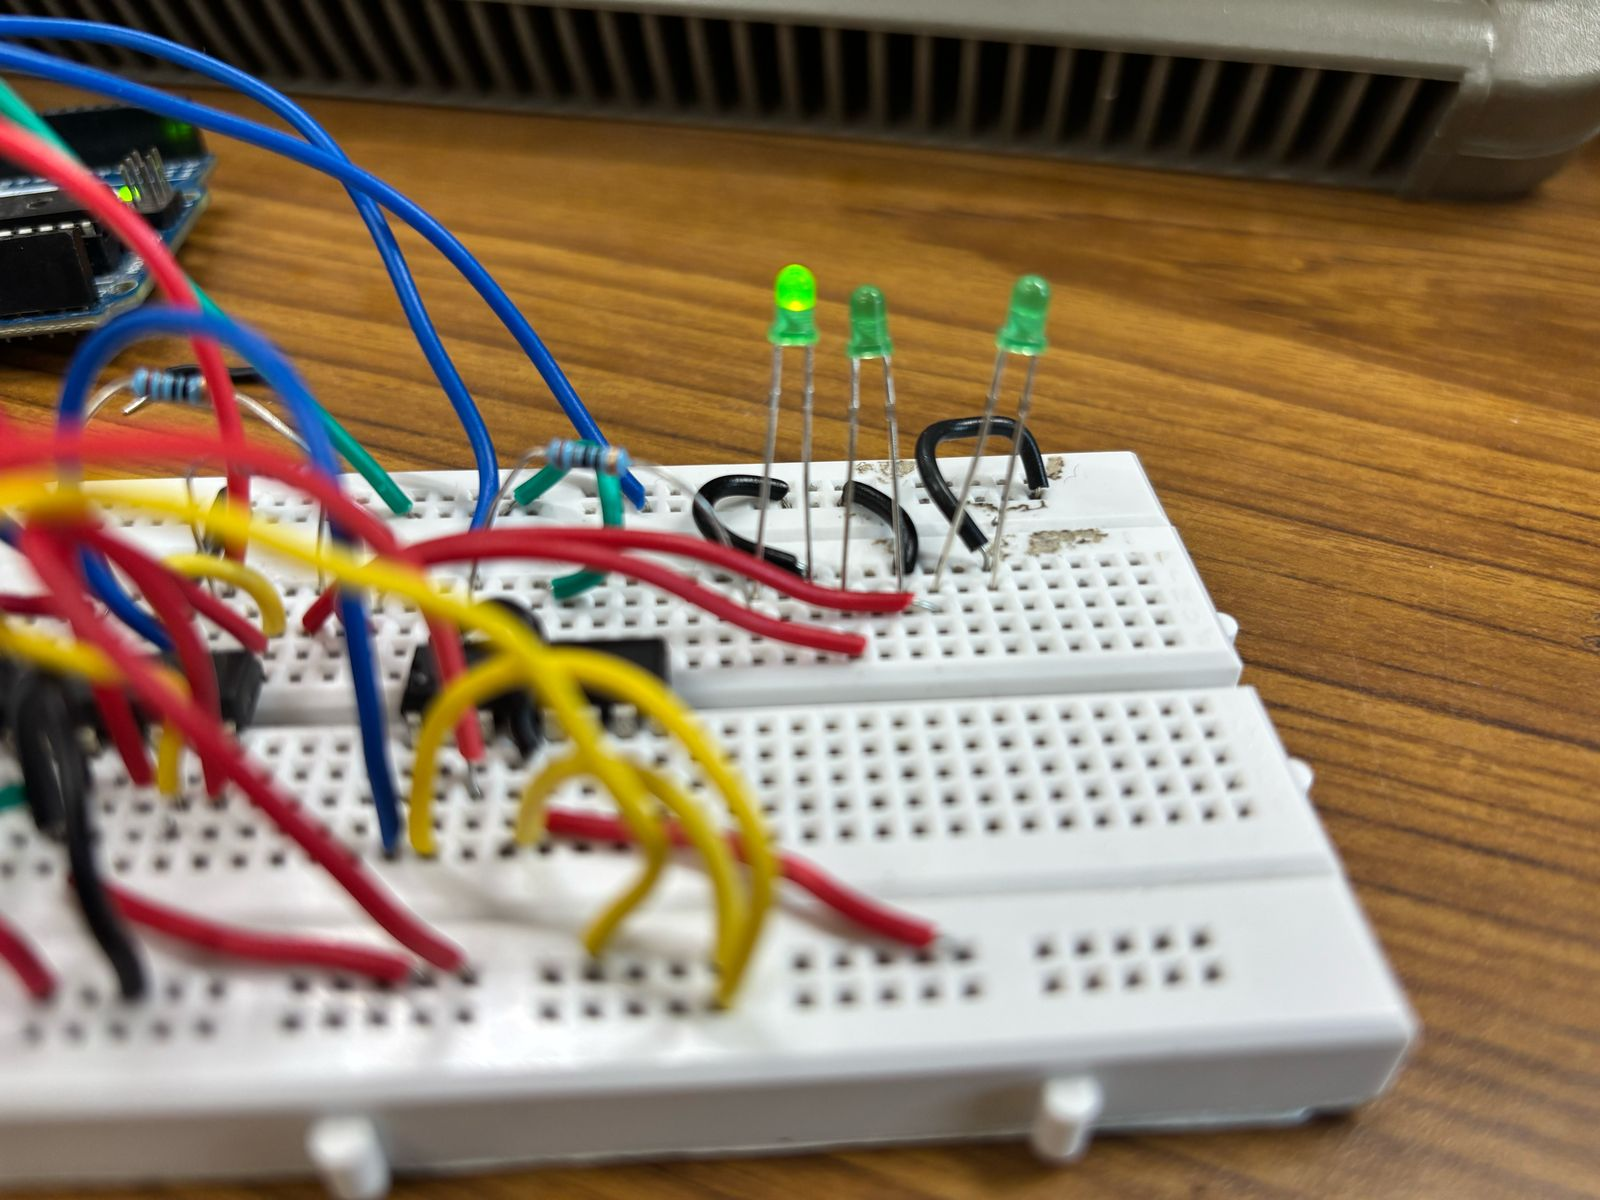
\includegraphics[width = 200pt]{figs/4.png}
	\end{subfigure}
	\hspace{110pt}
	\begin{subfigure}[b]{100pt}
		\caption{5}
		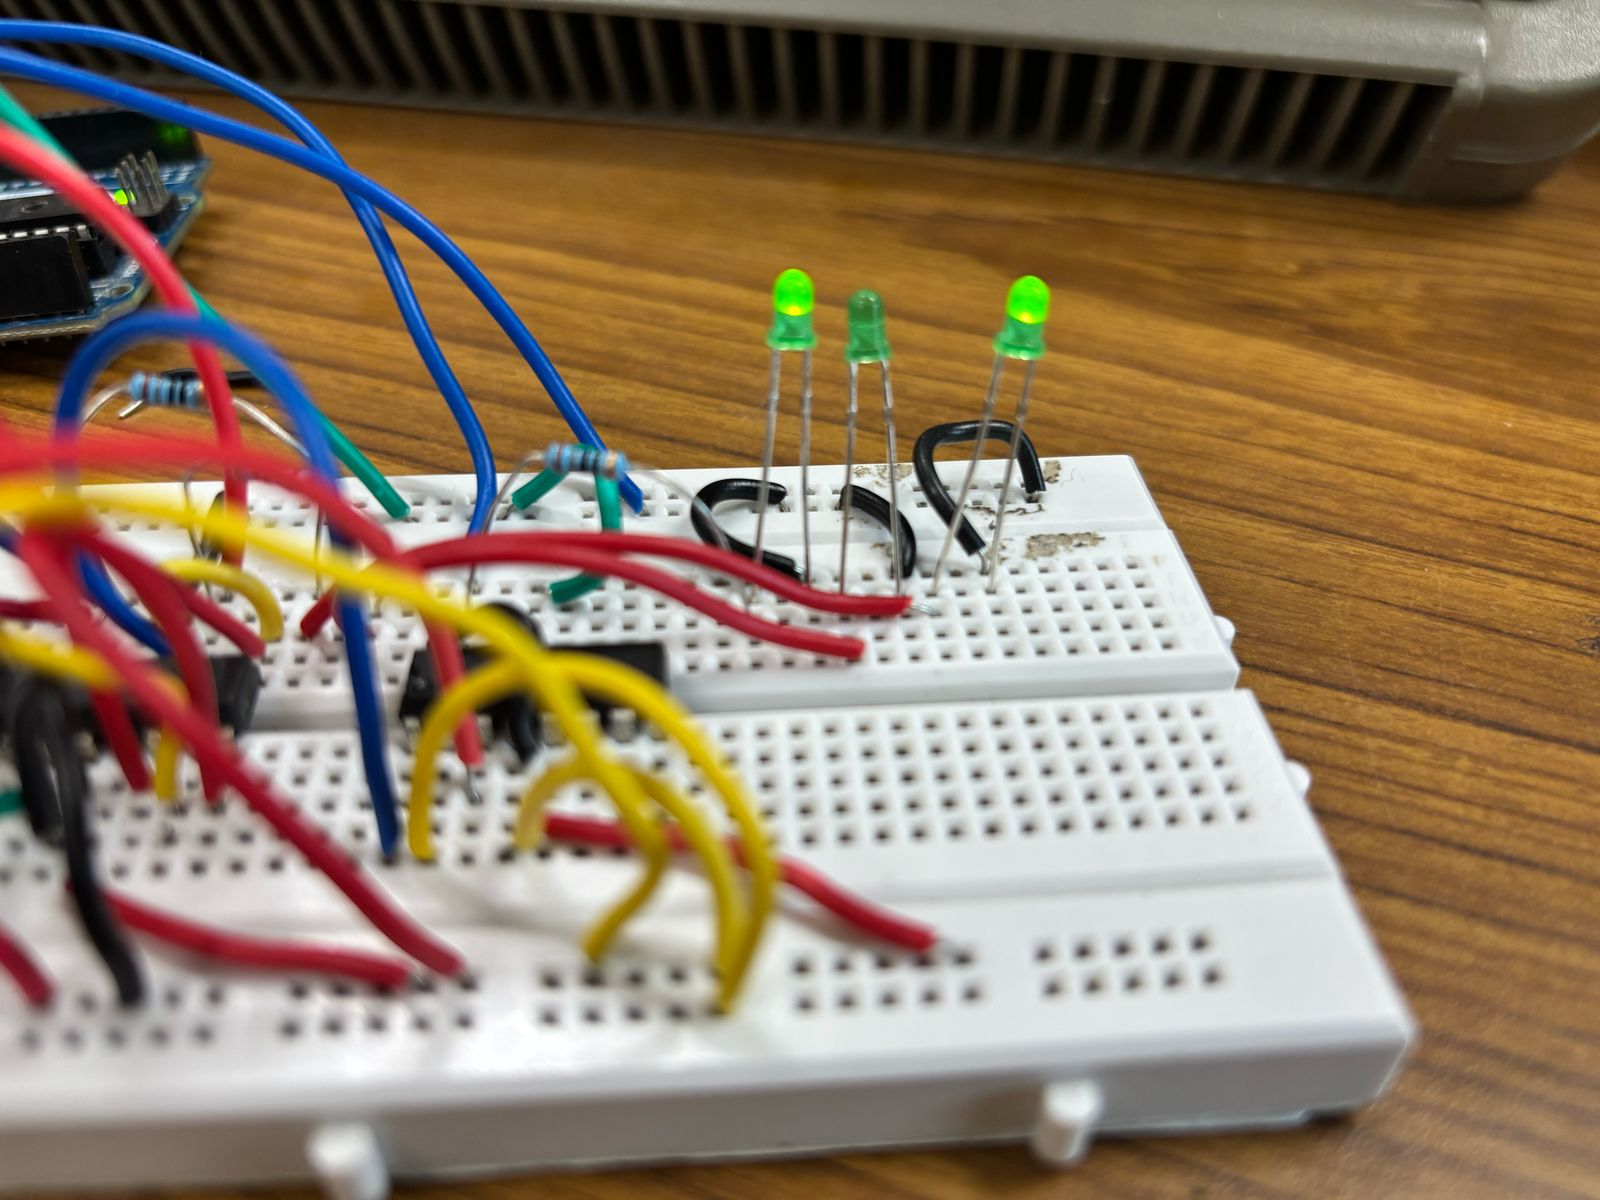
\includegraphics[width = 200pt]{figs/5.png}
	\end{subfigure}
    \begin{subfigure}[b]{100pt}
    \centering
		\caption{6}
		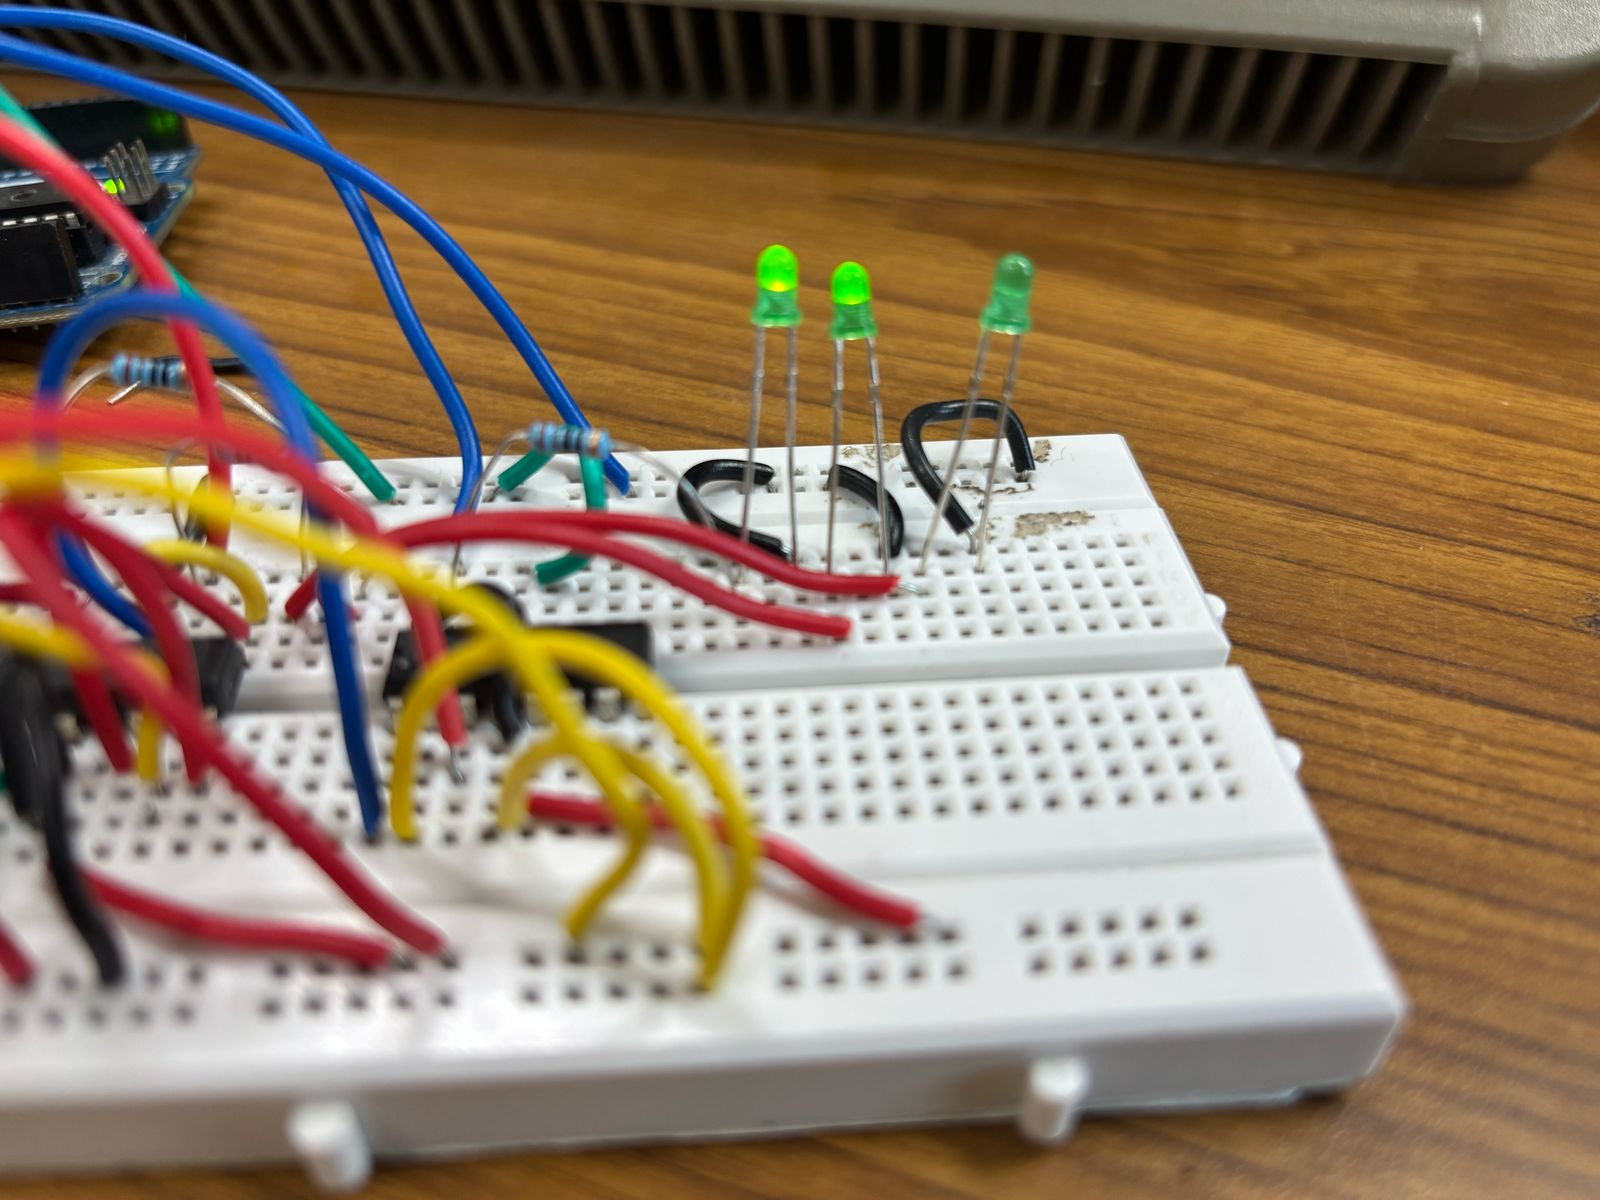
\includegraphics[width = 200pt]{figs/6.png}
	\end{subfigure}
	\hspace{110pt}
\end{figure}
\pagebreak
\begin{table}[h!]
\centering
\begin{tabular}{ccccc}
\toprule
Count & $Q_3$ & $Q_2$ & $Q_1$ & Decimal \\
\midrule
0 & 0 & 0 & 0 & 0 \\
1 & 0 & 0 & 1 & 1 \\
2 & 0 & 1 & 0 & 2 \\
3 & 0 & 1 & 1 & 3 \\
4 & 1 & 0 & 0 & 4 \\
5 & 1 & 0 & 1 & 5 \\
6 & 1 & 1 & 0 & 6 \\
7 & 0 & 0 & 0 & 0 \\
\bottomrule
\end{tabular}
\caption{Counting sequence of the Mod-7 counter}
\label{tab:counting_sequence}
\end{table}
\subsection{Oscilloscope Readings}
\begin{figure}[h!]
        \centering
		\caption{Oscilloscope Reading-1}
		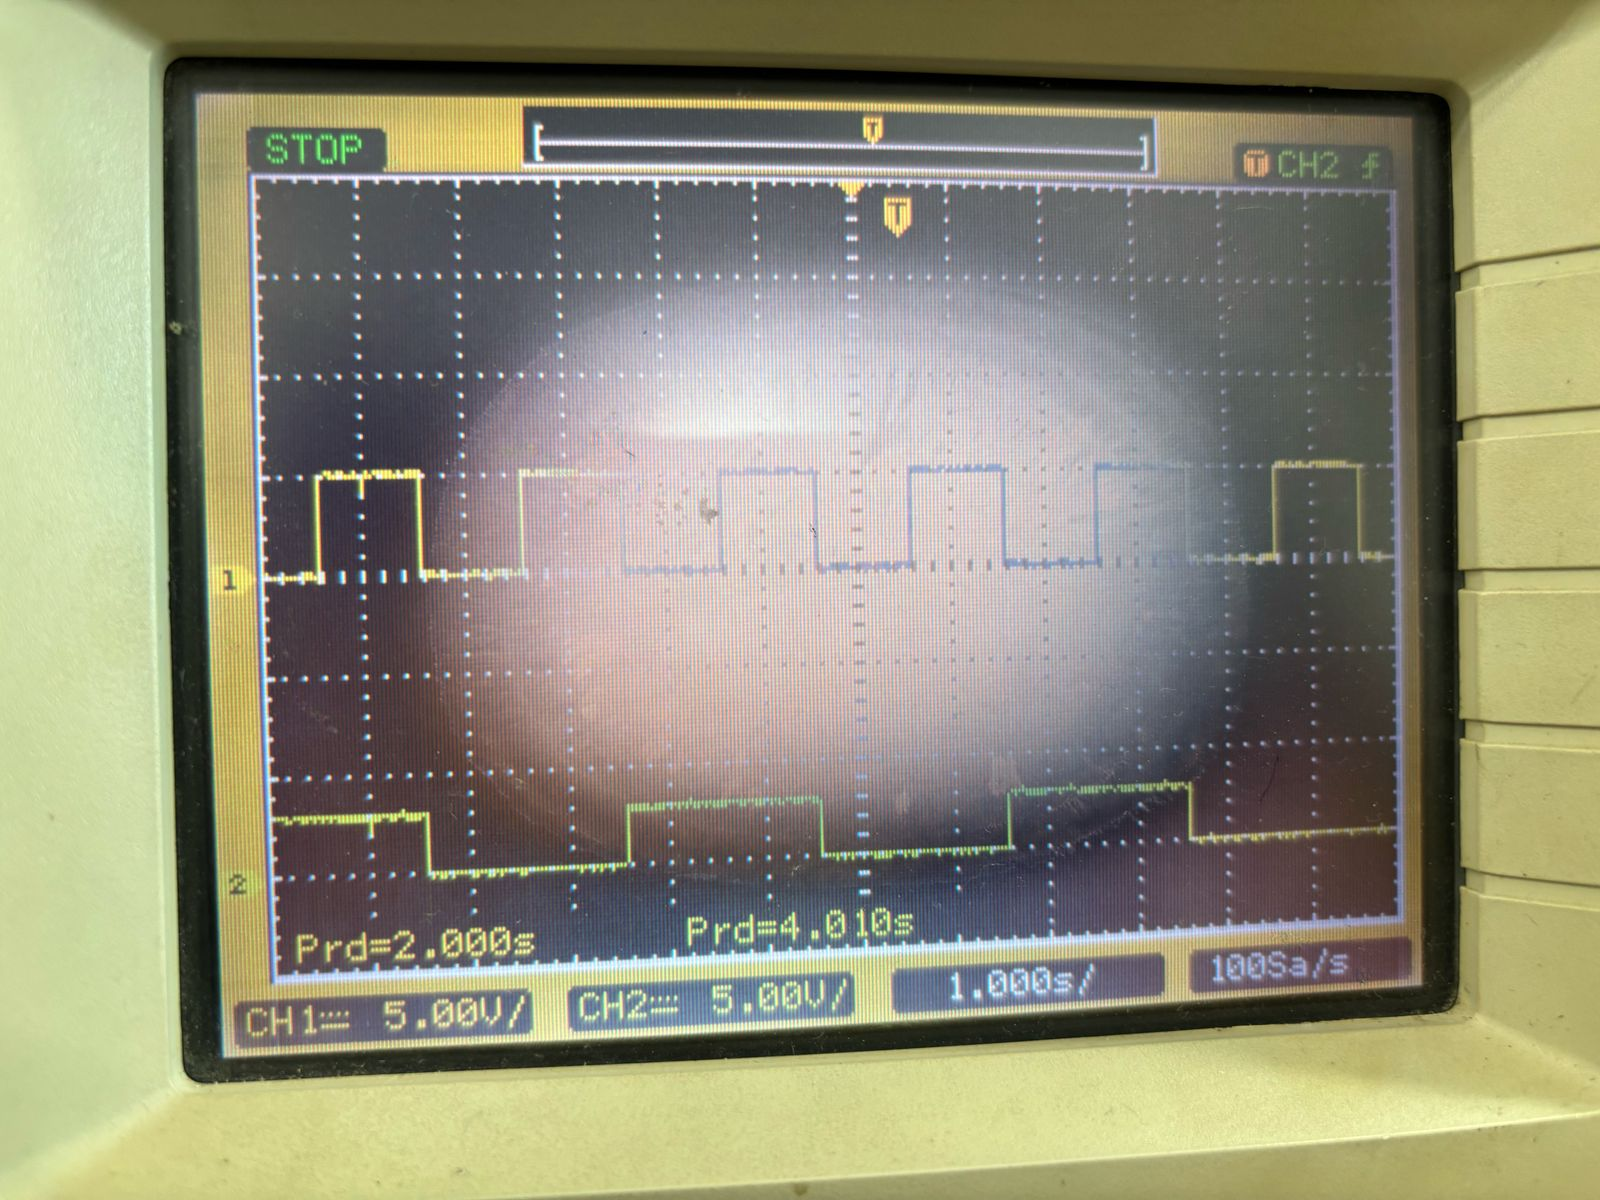
\includegraphics[width = 230pt]{figs/clk_vs_flipflop-1.png}
\end{figure}
\pagebreak
\begin{figure}[h!]
        \centering
		\caption{Circuit-1}
		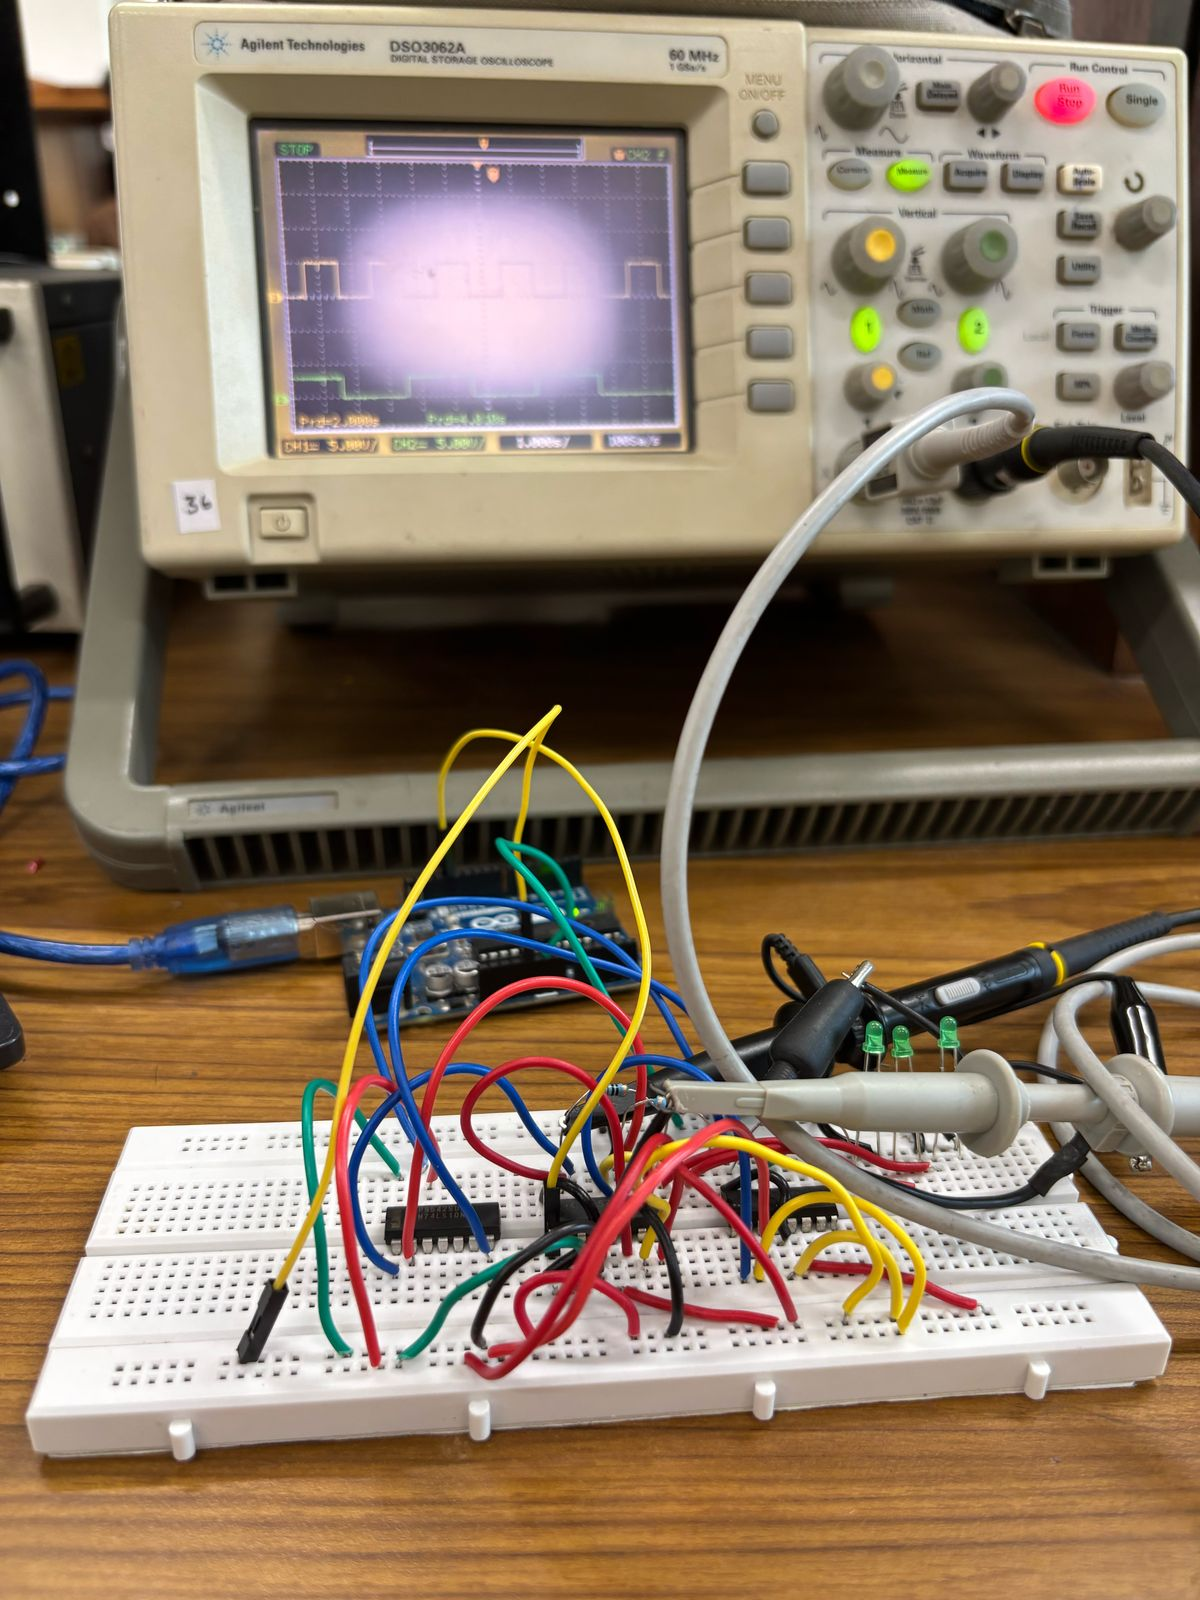
\includegraphics[width = 200pt]{figs/ckt_oscilloscope-1.png}
\end{figure}
\begin{figure}[h!]
        \centering
		\caption{Oscilloscope Reading-2}
		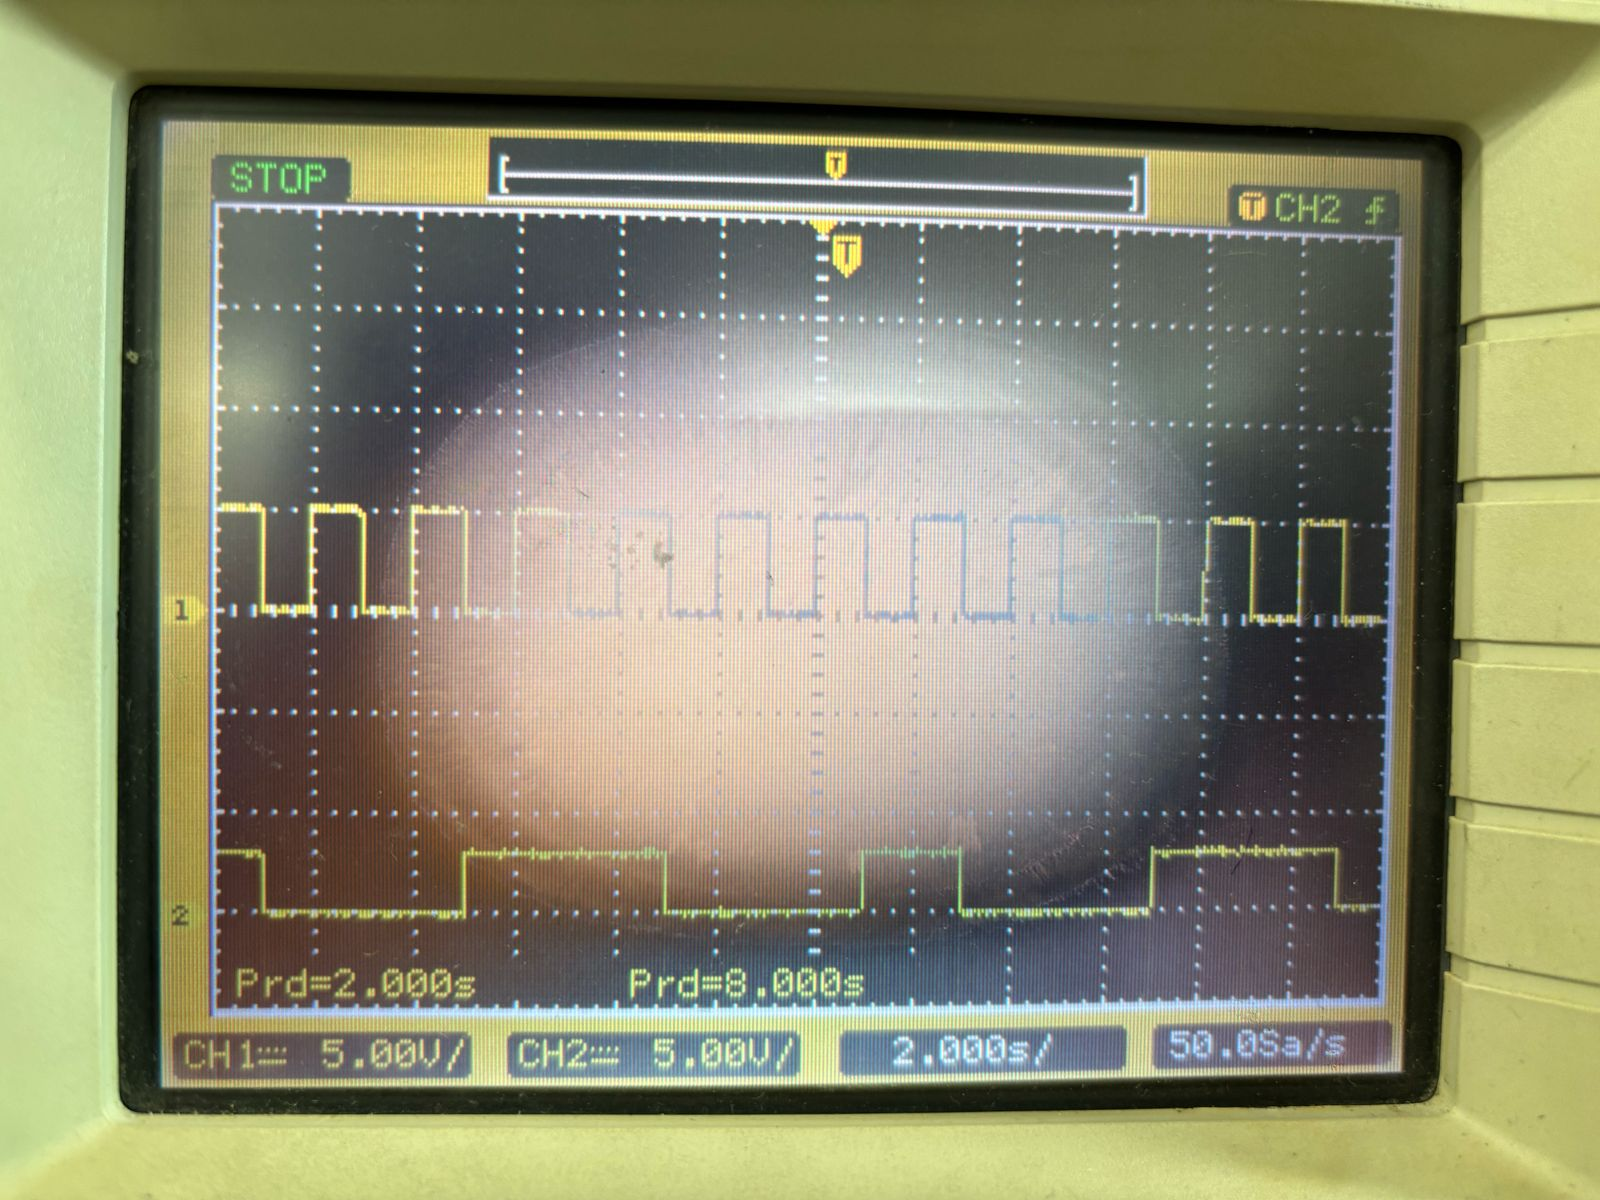
\includegraphics[width = 230pt]{figs/clk_vs_flipflop-2.png}
\end{figure}
\begin{figure}[h!]
        \centering
		\caption{Circuit-2}
		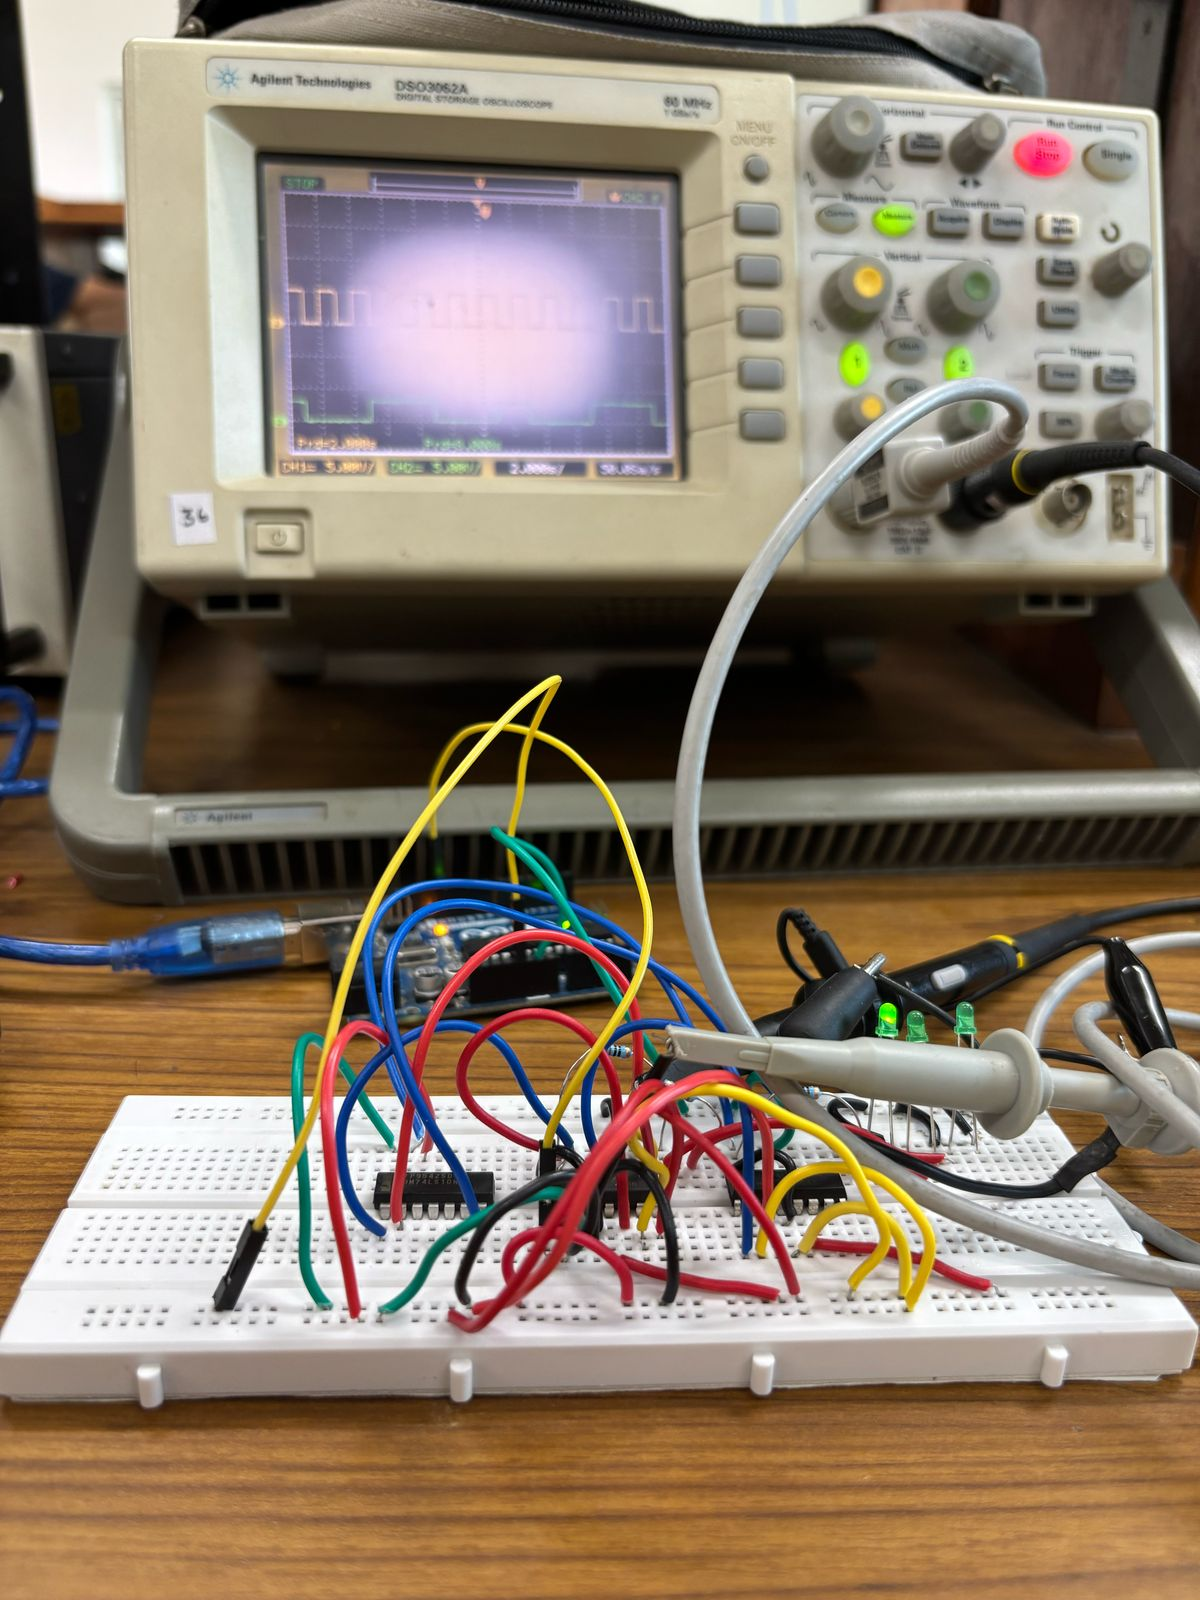
\includegraphics[width = 200pt]{figs/ckt_oscilloscope-2.png}
\end{figure}
\begin{figure}[h!]
        \centering
		\caption{Oscilloscope Reading-3}
		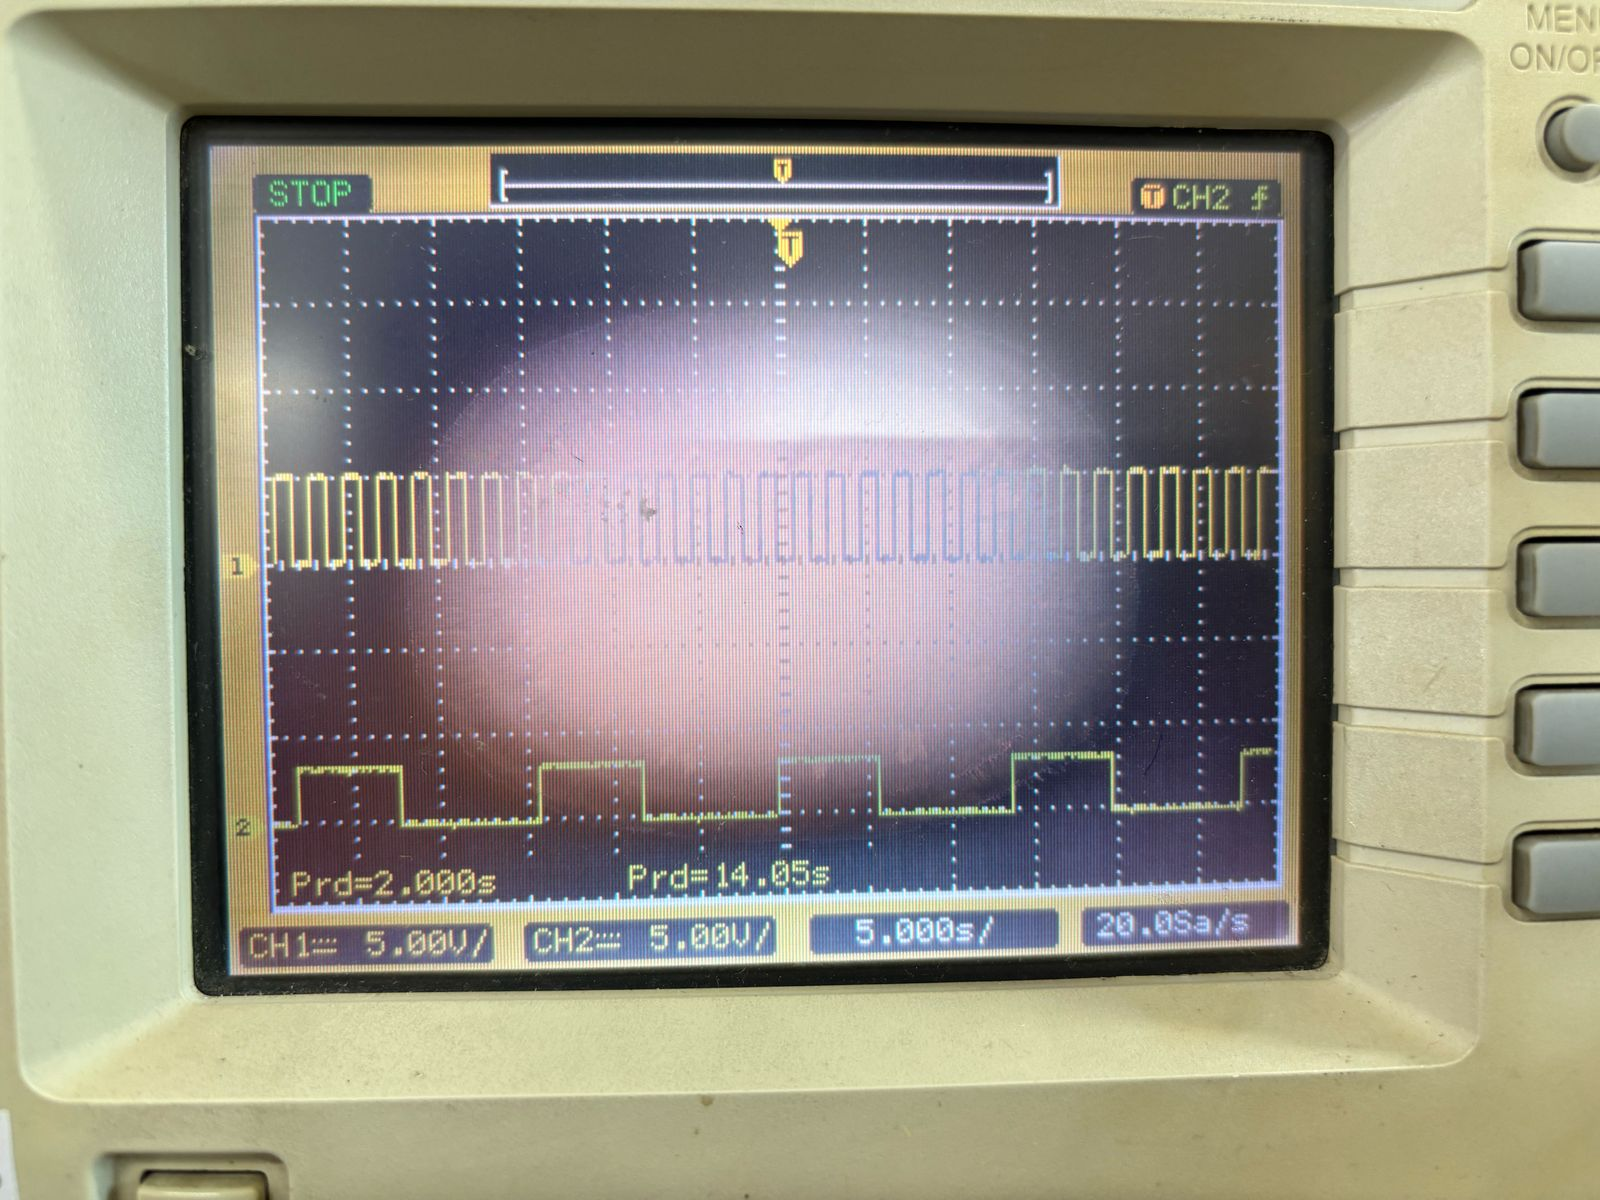
\includegraphics[width = 230pt]{figs/clk_vs_flipflop-3.png}
\end{figure}
\begin{figure}[h!]
        \centering
		\caption{Circuit-3}
		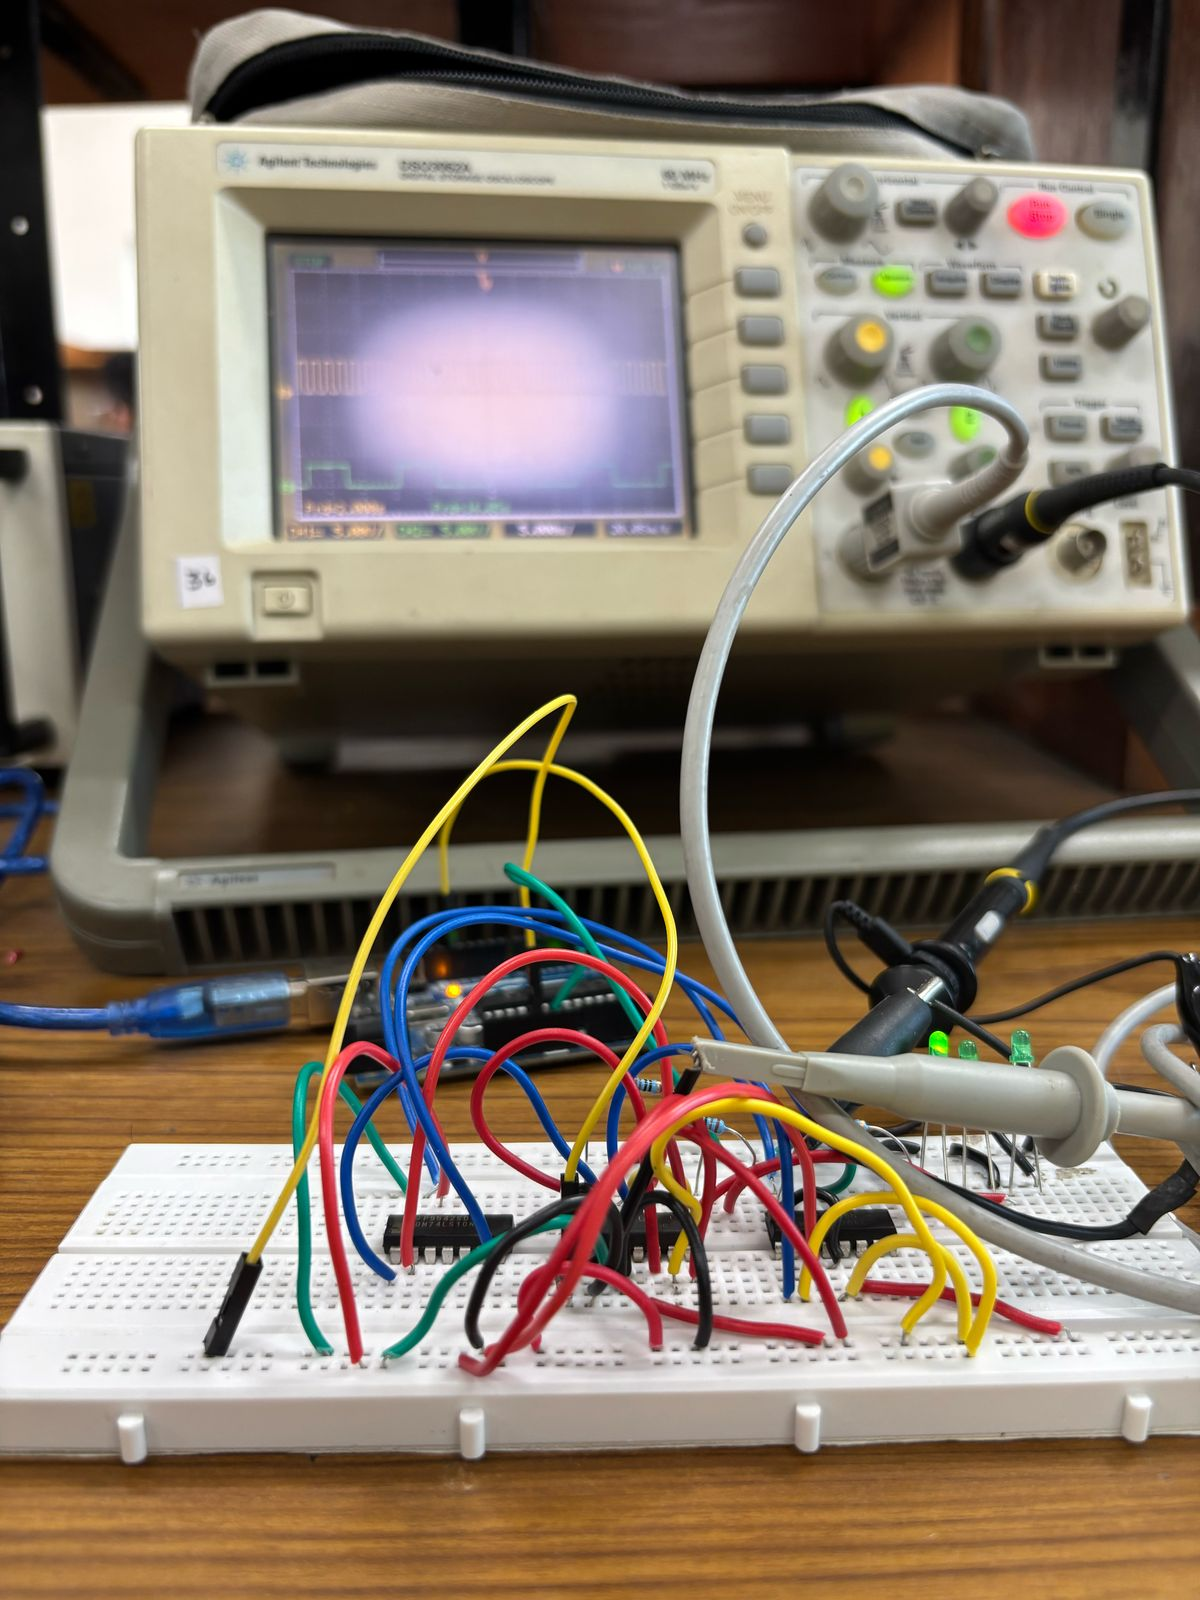
\includegraphics[width = 200pt]{figs/ckt_oscilloscope-3.png}
\end{figure}

\section{Conclusion}
The experiment successfully demonstrated the design and implementation of a Mod-7 asynchronous counter using T flip-flops converted from JK flip-flops, using Arduino as a clock.
\end{document}
